\documentclass[11pt]{article}
\usepackage{fullpage}
\usepackage{amsmath,amssymb}
\usepackage{graphicx}
\usepackage{color}
\usepackage{algorithm}
\usepackage{algcompatible}
\usepackage[colorlinks,bookmarksopen,bookmarksnumbered,citecolor=red,urlcolor=red,breaklinks=true]{hyperref}
\newcommand{\cblue}[1]{{\color{blue}#1}}
\renewcommand{\vec}[1]{{#1}}
\newcommand{\figdir}{./figures/}
\newcommand{\note}[1]{\cblue{NOTE: #1}}
\author{Eike Mueller, University of Bath}
\title{Multilevel Monte Carlo for Quantum Field Theories on the Lattice}
\begin{document}
\maketitle
%%%%%%%%%%%%%%%%%%%%%%%%%%%%%%%%%%%%%%%%%%%%%%%%%%%%%%%%%%%%%%%%%%%%%%%%%%%%
\section{Challenge and Motivation}
%%%%%%%%%%%%%%%%%%%%%%%%%%%%%%%%%%%%%%%%%%%%%%%%%%%%%%%%%%%%%%%%%%%%%%%%%%%%
Quantum Field Theories (QFTs) \cite{Peskin1995}, such as Quantum Chromo Dynamics (QCD) predict fundamental properties of subnuclear matter and are of paramount importance in High Energy Physics. If discretised on a space-time lattice, QCD allows first principles calculations of strongly interacting particles and is crucial for precise calculations, for example in New Physics predictions or to simulate the hadronic background in accelerators such as the Large Hadron Collider. 
Due to the strong coupling of QCD at large distances, only lattice calculations allow first-principles predictions, but they are computationally demanding. Using Feynman's Path Integral technique \cite{Feynman2010}, QFTs can be be formulated as statistical systems in $d=4$ space-time dimensions. Predictions of physical quantities are then calculated by generating a set of samples with Markov-Chain Monte Carlo Methods. The relevant quantity of interest (such as a two-point correlation function, which allows the extraction of particle energies) is then evaluated on those samples. To obtain physically meaningful results, calculations need to be carried out for increasingly small lattice spacings $a$ and extrapolated to the continuum limit $a\rightarrow 0$, which can amplify sampling errors. There are two fundamental issues which make accurate numerical calculations challenging:
\begin{figure}
  \begin{center}
    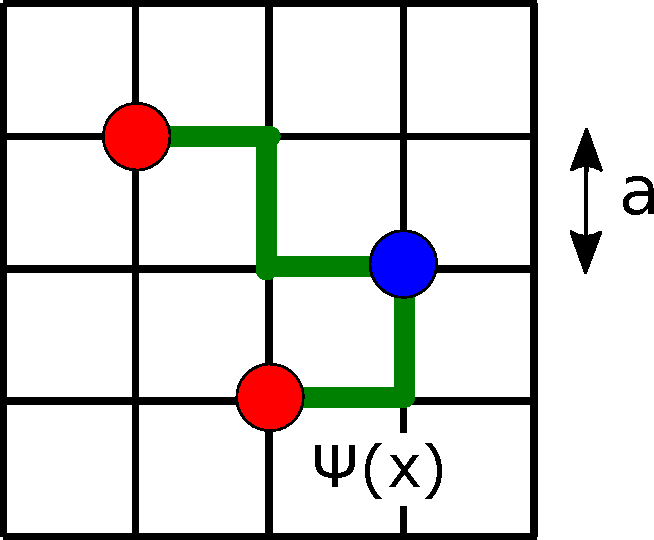
\includegraphics[width=0.3\linewidth]{\figdir/lattice.pdf}
    \caption{Fields on a space-time lattice}
    \label{fig:lattice}
  \end{center}
\end{figure}
\begin{itemize}
\item Since the probability density is peaked around the classical trajectory, in the Metropolis-Hastings algorithm naively generated samples are highly correlated since the acceptance probability is small. This issue can be overcome by the Hybrid Monte Carlo method \cite{Duane1987}. However, the number of samples $N$ required to reduce the statistical sampling error below a tolerance $\epsilon$ still grows as $\mathcal{O}(\epsilon^{-2})$ due to fundamental law of large numbers. 
\item Since the number $M$ of lattice sites on a grid with spacing $a$ is $M \propto a^{-d}$, the cost to generate one sample grows as $\mathcal{O}(a^{-d})$. This already assumes that optimal algorithms are used when, for example, inverting large sparse matrices to calculate Fermion propagators, which is usually the computational bottleneck in unquenched simulations (see e.g. \cite{Brannick2008} on multigrid methods). While most theories are formulated in $d=3+1=4$ spacetime dimensions, in some case (such as Domain Wall Fermions \cite{Kaplan1992}) the dimension of the system is even $d=5$.
\end{itemize}
We assume that the discretisation error is linear in the lattice spacing. Note that as discussed in \cite{Lepage1994}, for a quantum field theory this is only true if the theory is renormalised correctly. If both the statistical and discretisation error are to be reduced below a tolerance of $\epsilon\propto a$, the total cost of the method is \mbox{$\mathcal{O}(N\cdot M) = \mathcal{O}(\epsilon^{-(d+2)})$} where $d=4,5$. Together this leads to prohibitively high costs for Lattice QCD calculations which limit the range of available lattice spacings and extrapolations to the continuum limit. Since the lattice calculation is carried out in a finite volume, this introduces an additional error, which is, however, suppressed exponentially like
\begin{equation}
  \text{(finite volume error)} \propto \exp\left[-m_\pi L\right]\label{eqn:finite_size}
\end{equation}
where $L$ is the size of the simulation box and $m_\pi$ is the mass of the lightest hardron (i.e. the pion) \cite{Lepage1994}.

Typical lattice sizes and sample numbers can be found in \cite{Bazavov2013} where the authors of the MILC collaboration report on the generation of ensembles with an improved quark action. As table 1 in \cite{Bazavov2013} shows, the largest lattices consist of $96^3\times 192$ points and $\sim 1,000$ independent gauge configurations are created. The lattice spacing of those largest configurations is $\approx 0.06\operatorname{fm}$ and the pion mass $135 \operatorname{MeV}$, the reported value of $m_\pi L$ which enters in Eq. (\ref{eqn:finite_size}) is $m_\pi L=3.95$.
\note{This paper is nearly 5 years old now, so numbers might have changed a bit, but unlikely they have gone up by more than a factor two or so.}
Five-dimensional domain-wall fermion simulations use even larger lattice spacings with $32^3\times 64\times 12$ or $24^3\times 64\times 24$ lattice sites \cite{Jung2017}.
%%%%%%%%%%%%%%%%%%%%%%%%%%%%%%%%%%%%%%%%%%%%%%%%%%%%%%%%%%%%%%%%%%%%%%%%%%%%
\subsection{Multilevel Monte Carlo and renormalisation}
%%%%%%%%%%%%%%%%%%%%%%%%%%%%%%%%%%%%%%%%%%%%%%%%%%%%%%%%%%%%%%%%%%%%%%%%%%%%
In the following we explore Multilevel Monte Carlo sampling methods \cite{Heinrich2001,Giles2008,Giles2015}. As shown in \cite{Dodwell2015}, a Multilevel MCMC method has the potential to reduce the computational complexity from $\mathcal{O}(\epsilon^{-(d+2)})$ to $\mathcal{O}(\epsilon^2 |\log(\epsilon)|)$. Multilevel Monte Carlo uses a hierarchy of levels to construct an unbiased estimator. This requires calculation of the expectation value of differences $Y_\ell$ between subsequent levels $\ell$ and $\ell-1$, which have a much smaller variance than the QoI itsself. An important requirement is that the theories used on two subsequent levels are ``close'', i.e. the coarse level theory should provide a good approximation for the coarse modes on the next-finer level. In QFT this can be achieved naturally by constructing the coarse theory as an effective theory of the fine-level model. While construction of the exact effective theory by integrating out the high-frequency modes is not possible (except in very simple toy models), in many cases perturbation theory can be used to construct an approximate effective theory. In particular we expect this to be the case for fine lattice spacings $a$ in QCD, since the theory is asymptotically free (i.e. the strong coupling constant decreases as $a\rightarrow 0$). More specifically, at lowest order in perturbation theory the coupling constant $\alpha_s$ depends on the momentum scale $Q$ as
\begin{equation}
  \alpha_s(Q) = \frac{4\pi}{\beta_0 \log(Q^2/\Lambda^2)}
\end{equation}
where $\Lambda$ is a scale and $\beta_0=11-\frac{2}{3}n_f>0$ provided the number of fermions is $n_f\le 16$. Since due to the uncertainty principle a momentum is inverse related to a distance $a\sim 1/Q$, the coupling constant decreases logarithmically with the distance $a$ as
\begin{equation}
  \alpha_s(a) \sim \frac{1}{|\log(a^2\Lambda^2)|}.
\end{equation}
A whole machinery is available for carrying out perturbation theory on a lattice, see e.g. \cite{Rothe2005,Hart2009}.
\begin{figure}
\begin{center}
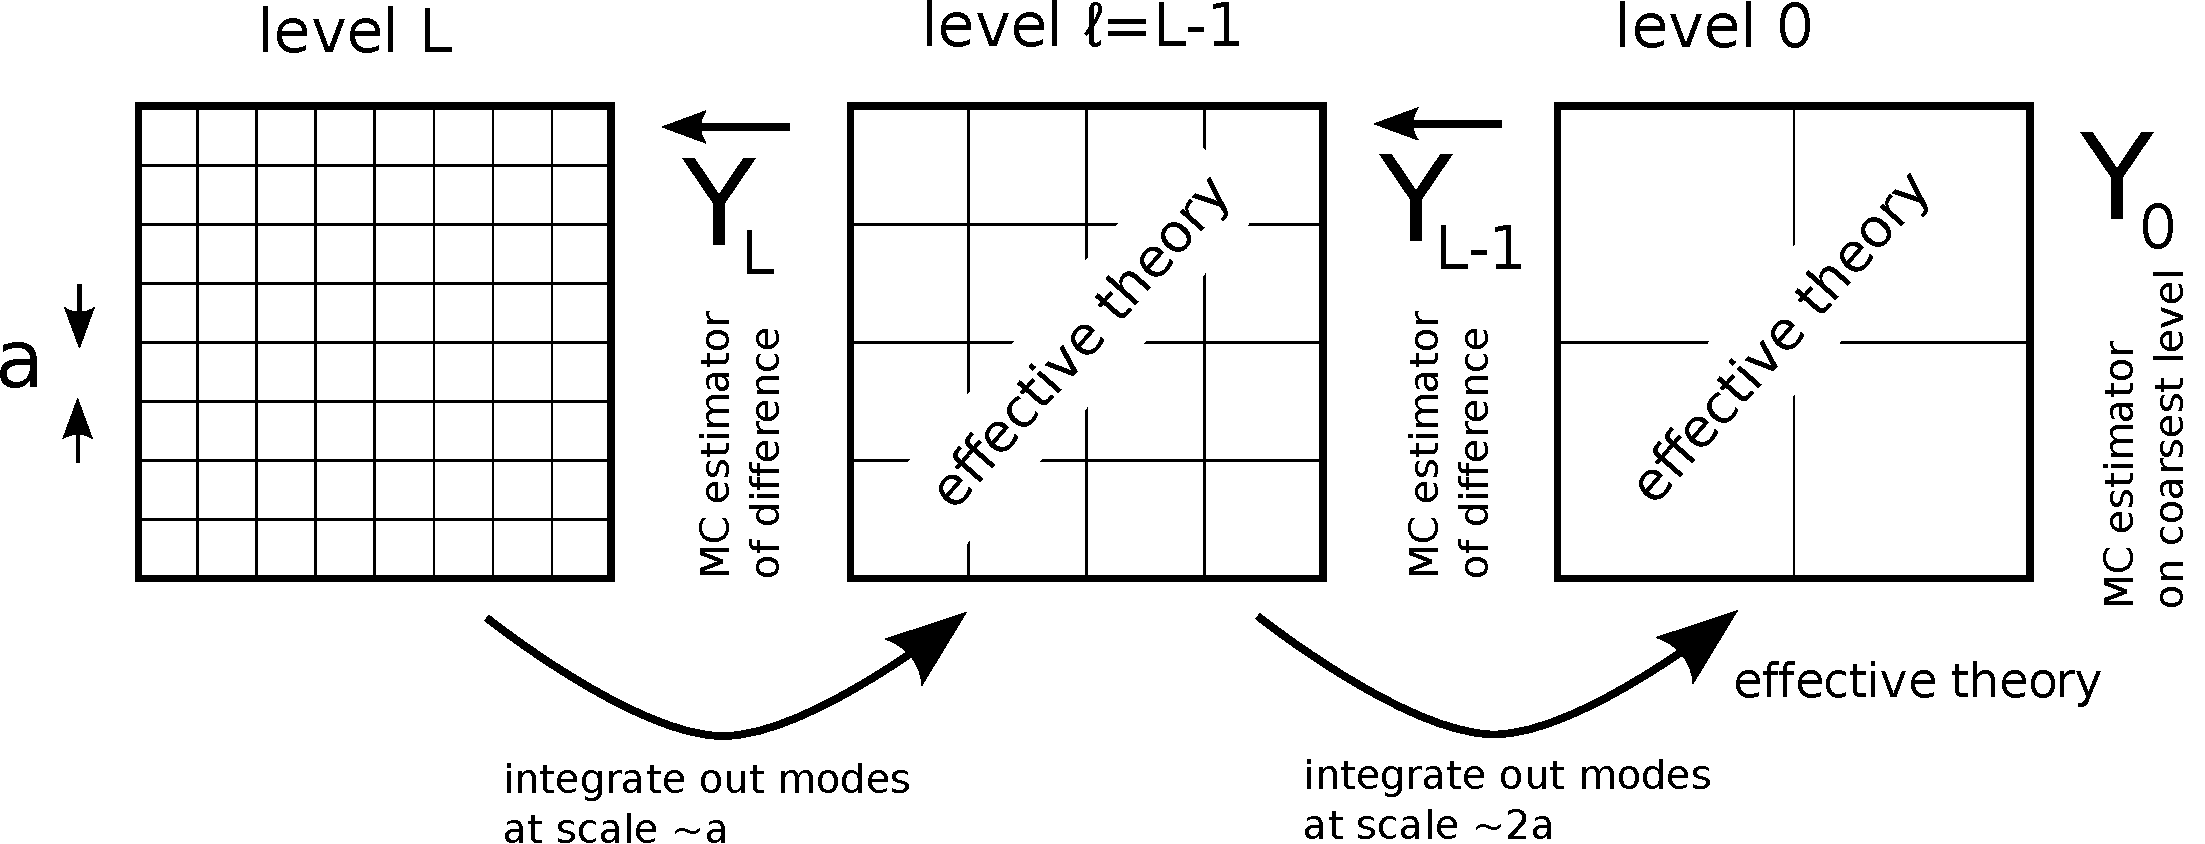
\includegraphics[width=0.9\linewidth]{\figdir/multilevel_schematic.pdf}
\caption{Schematic multilevel algorithm}
\label{fig:multilevel_schematic}
\end{center}
\end{figure}
Multilevel sampling also avoids strong correlation of subsequent samples in the MCMC chains (which is traditionally overcome with the HMC algorithm) since the samples are constructed hierarchically. The next proposal states on a level takes into account all fluctuations on the coarser levels.

More generally, renormalisation theory provides a tool for the systematic construction of coarse grained theories. It also applies to statistical systems (such as the Ising- or Heisenberg-model) and is important for the study of critical phenomena. One key observation here is that close to a critical point the theory is scale invariant, and again it is possible to write down a coarse grained version. This is interesting, because sampling at a critical point suffers from critical slowdown, yet this is exactly the point where the coarse-level theory is known and multilevel methods are expected to be efficient. In the past, hierarchical sampling techniques have been developed for the Ising model \cite{Schmidt1983,Faas1986}, but they do not exploit the additional variance reduction from the multilevel algorithm.
%%%%%%%%%%%%%%%%%%%%%%%%%%%%%%%%%%%%%%%%%%%%%%%%%%%%%%%%%%%%%%%%%%%%%%%%%%%%
\section{Methods}
%%%%%%%%%%%%%%%%%%%%%%%%%%%%%%%%%%%%%%%%%%%%%%%%%%%%%%%%%%%%%%%%%%%%%%%%%%%%
To set the scene and introduce key concepts, we first discuss the much simpler case of quantum mechanics and show how it can be formulated as a statistical theory. As an instructive example, the derivation of an effective theory for the quantum mechanical harmonic oscillator is described in appendix \ref{sec:harmonic_oscillator_effective}.

Since quantum mechanics is effectively a one-dimensional field-theory, the gains are expected to be smaller here ($\mathcal{O}(\epsilon^{-3})\rightarrow\mathcal{O}(\epsilon^{-2}|\log(\epsilon)|)$). We discuss the generalisations required for the more interesting case of a $d$-dimensional Quantum Field Theory in Section \ref{sec:QFT}. 
%%%%%%%%%%%%%%%%%%%%%%%%%%%%%%%%%%%%%%%%%%%%%%%%%%%%%%%%%%%%%%%%%%%%%%%%%%%%
\subsection{Path integrals in Quantum Mechanics}
%%%%%%%%%%%%%%%%%%%%%%%%%%%%%%%%%%%%%%%%%%%%%%%%%%%%%%%%%%%%%%%%%%%%%%%%%%%%
Consider a particle of mass $m_0$ which moves in a potential $V(x)$ where $x(t)$ is the particle's position at time $t$.
Feynman's path integral \cite{Feynman2010} allows the calculation of the quantum mechanical transition amplitude for starting at the point $x_i$ at time $t=0$ and ending at point $x_f$ at time $t=T$ as a sum over all possible paths $x(t)$ with $x(0)=x_i$,  $x(T)=x_f$, denoted by the integral
\begin{equation} 
\sum_{\text{all paths $x(t)$}}\leftrightarrow  \int \mathcal{D}x(t).
\end{equation}
This is shown schematically in Fig. \ref{fig:path_integral} (left)\footnote{The figure is slightly misleading since the paths are continuous but not necessarily smooth (differentiable).}. The crucial observation, exploited for example in \cite{Creutz1981}, is that by formulating the theory in imaginary time, the highly-oscillatory integrand is replaced by a real exponential and the path integral is equivalent to a statistical system of temperature\footnote{In the ``zero-temperature'' limit quantum fluctuations disappear and only the classical trajectory which minimises the action in Eq. (\ref{eqn:action}) contributes to the path integral.} proportional to Planck's constant $\hbar$.  The transition amplitude is given by
\begin{equation}
  \mathcal{A}(x_f\leftarrow x_i)=\langle x_f| e^{-HT} |x_i\rangle = \int\mathcal{D}x(t)\;e^{-S[x(t)]}.\label{eqn:path_integral_continuum}
\end{equation}
For simplicity we have chosen units in which $\hbar=1$.
For a given path $x(t)$ the action $S[x(t)]$ is
\begin{equation}
  S[x(t)] = \int_{0}^{T} \left(\frac{1}{2}m_0 \dot{x}(t)^2 + V(x(t))\right)\;dt\label{eqn:action}
\end{equation}
\begin{figure}
  \begin{center}
    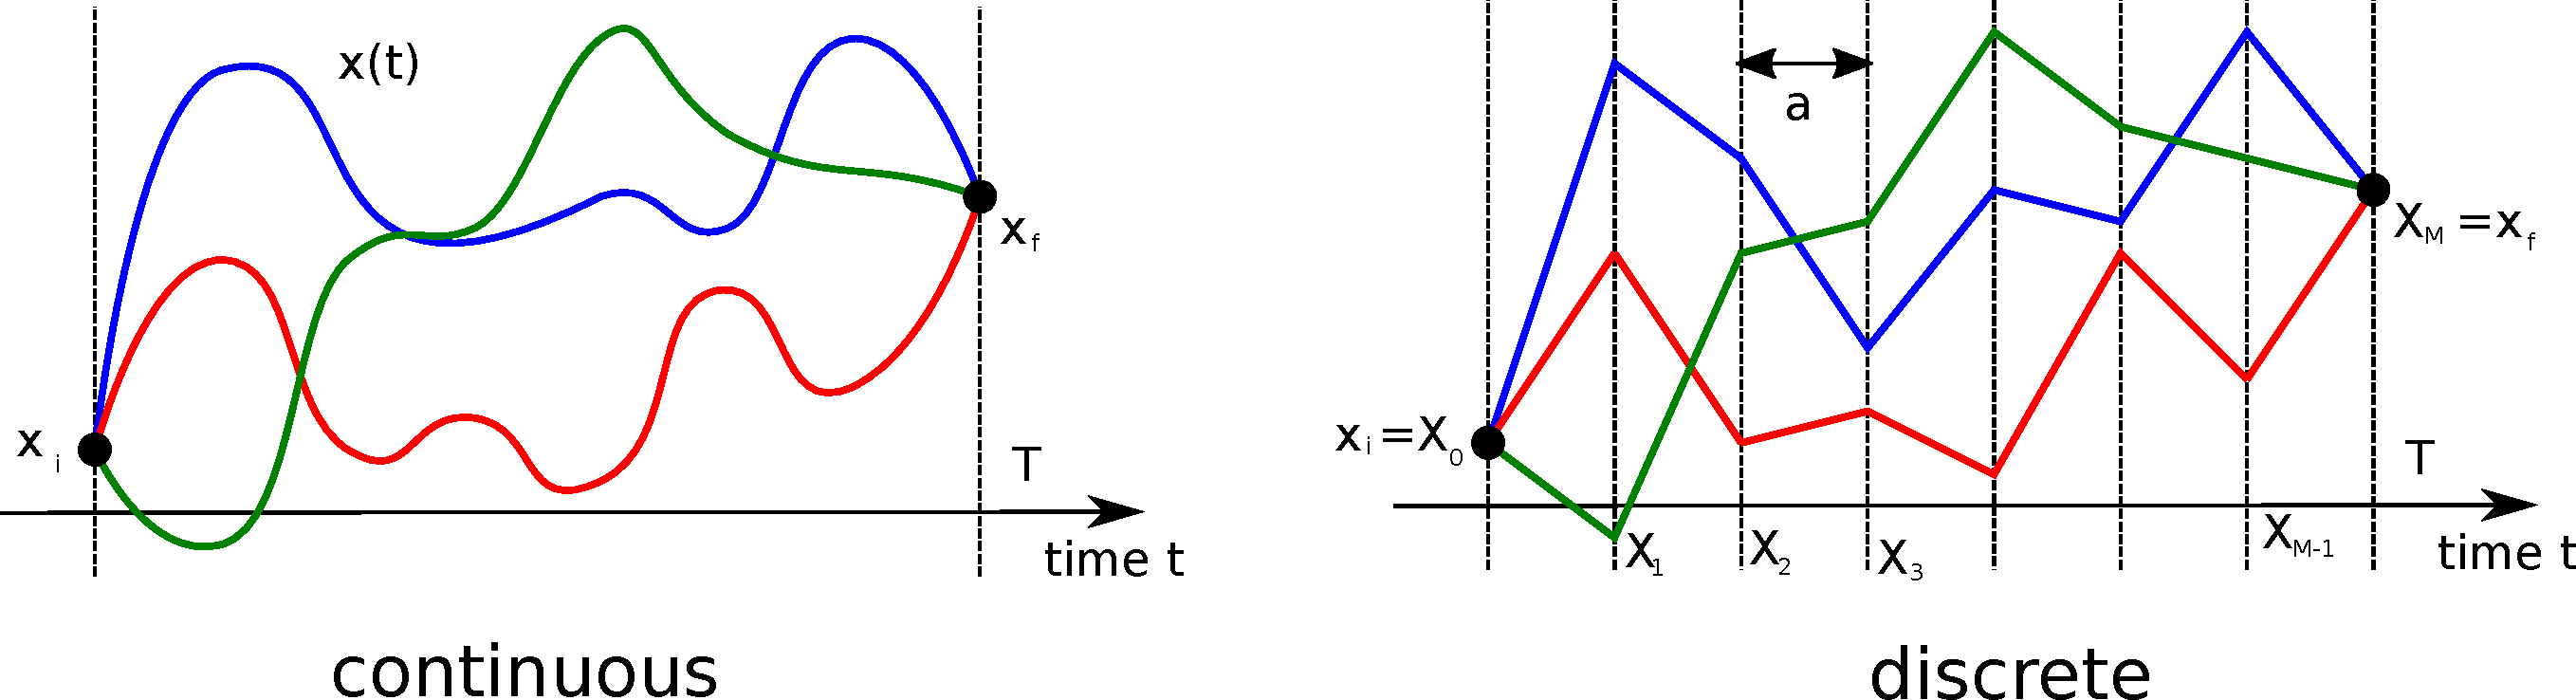
\includegraphics[width=\linewidth]{\figdir/path_integral.pdf}
    \caption{Path integral in the continuum (left) and on a time-lattice of spacing $a$ (right).}
    \label{fig:path_integral}
  \end{center}
\end{figure}
From now on we will also use periodic boundary conditions $x_i=x_f$ and integrate over $x_i$ as well in Eq. (\ref{eqn:path_integral_continuum}). This is much easier than using ``Dirichlet-like'' boundary conditions where the particle's position is fixed at $t=0$ and $t=T$; in the infinite-volume limit $T\rightarrow \infty$ the boundary conditions do not matter since the finite volume error is exponentially suppressed \cite{Lepage1994}.
Path-dependent observables $A=A[x(t)]$ (or ``quantities of interest'', QoIs) can be calculated as expectation values
\begin{equation}
  \langle A \rangle = \frac{\int \mathcal{D}x(t) A[x(t)] e^{-S[x(t)]}}{\int \mathcal{D}x(t) e^{-S[x(t)]}}\label{eqn:expectation_A}
\end{equation}
For example, the two-point correlation function $A=x(0)x(t)$ allows the extration of the system energies $E_n$ since it can be shown that\footnote{Strictly speaking only true if $\langle x(t)\rangle=0$, which is the case for symmetric potentials.}
\begin{equation}
  C(t) = \langle x(0) x(t) \rangle = \sum_{n\ne 0} C_n e^{-(E_n-E_0)t}.\label{eqn:spectrum}
\end{equation}
This formula is also crucial in QFT, for example in QCD it can be used to extract the mass-spectra of bound particle states by fitting the correlation function $C(t) = \langle x(0)x(t)\rangle$ to a sum of exponentials (see \cite{Fodor2012} for a review on how this is done). The theoretical predictions can then be compared to experimental data (see e.g. \cite{Davies2004}).

Using more abstract notation, we can express the expectation value of the observable $A$ in Eq. (\ref{eqn:expectation_A}) as
\begin{equation}
   \langle A \rangle = \mathbb{E}_{\rho}\left[A\right]
\end{equation}
where $\rho$ is the probability measure defined by
\begin{equation}
  \rho(x(t)) = \frac{e^{-S[x(t)]}}{Z}\mathcal{D}x(t)\qquad\text{with normalisation constant $Z = \int \mathcal{D}x'(t)\; e^{-S[x'(t)]}$}. \label{eqn:measure_continuum}
\end{equation}
%%%%%%%%%%%%%%%%%%%%%%%%%%%%%%%%%%%%%%%%%%%%%%%%%%%%%%%%%%%%%%%%%%%%%%%%%%%%
\subsubsection{Discretisation}
%%%%%%%%%%%%%%%%%%%%%%%%%%%%%%%%%%%%%%%%%%%%%%%%%%%%%%%%%%%%%%%%%%%%%%%%%%%%
Clearly the infinite dimensional integral in Eq. (\ref{eqn:expectation_A}) can not be calculated and needs to be replaced by a finite-dimensional approximation. To discretise, replace the path $x(t)$ by a finite number of points as shown in Fig. \ref{fig:path_integral} (right)
\begin{equation}
  x(t) \mapsto \vec{X} = (X_0,X_1,\dots,X_{M-1})\qquad\text{with $X_j=x(ja)$}.
\end{equation}
Here $a$ is the lattice spacing. The quantity $\vec{X}$ is the state vector of the system and the path integral is the sum over all states $X$ with an appropriate exponential weighting $e^{-S[X]}$.
More specifically, on the lattice the infinite dimensional integral in Eq. (\ref{eqn:expectation_A}) becomes the $M$-dimensional integral
\begin{equation}
  \langle A\rangle \approx \frac{\int d^M\vec{X} \;A[X]e^{-S[\vec{X}]}}{\int d^M\vec{X'} \;e^{-S[\vec{X'}]}}
  \qquad\text{where $d^M\vec{X}=dX_0\;dX_1\;\dots\;dX_{M-1}$}\label{eqn:generating_functional_disc}
\end{equation}
with the discretised action\footnote{Obviously, other discretisations could be used for the time derivative $\dot{x}(t)$.}
\begin{equation}
  S[\vec{X}] = \sum_{j=0}^{M-1} a \left(\frac{1}{2}m_0\frac{(X_{j+1}-X_j)^2}{a^2}+V(X_j)\right)\label{eqn:action_discrete}
\end{equation}
This integral is solved exactly for the quantum mechanical harmonic oscillator $V(x)=\frac{1}{2}m_0\mu^2 x^2$ in \cite{Creutz1981} (see also appendix \ref{sec:harmonic_oscillator}), i.e. in this case we know the bias (and also any finite volume errors).

In general, for a QFT on a $d$-dimensional space-time lattice Eq. (\ref{eqn:generating_functional_disc}) is a $M\propto a^{-d}$ dimensional integral. Replacing Eq. (\ref{eqn:expectation_A}) by Eq. (\ref{eqn:generating_functional_disc}) introduces a bias $a^{\kappa} \propto M^{-\alpha}$ where $\alpha=\kappa/d$, see \cite{Lepage1994} for a careful discussion of errors in QFT.
%%%%%%%%%%%%%%%%%%%%%%%%%%%%%%%%%%%%%%%%%%%%%%%%%%%%%%%%%%%%%%%%%%%%%%%%%%%%
\subsection{Sampling with Markov chains}
%%%%%%%%%%%%%%%%%%%%%%%%%%%%%%%%%%%%%%%%%%%%%%%%%%%%%%%%%%%%%%%%%%%%%%%%%%%%
%%%%%%%%%%%%%%%%%%%%%%%%%%%%%%%%%%%%%%%%%%%%%%%%%%%%%%%%%%%%%%%%%%%%%%%%%%%%
\subsubsection{MCMC sampling}
%%%%%%%%%%%%%%%%%%%%%%%%%%%%%%%%%%%%%%%%%%%%%%%%%%%%%%%%%%%%%%%%%%%%%%%%%%%%
For a general potential $V(x)$ expectation values can not be calculated directly. Instead, we use MCMC estimators to evaluate the high-dimensional integral in Eq. (\ref{eqn:generating_functional_disc}). We first ensure that the notation is consistent with \cite{Dodwell2015}. For this, observe that since (in contrast to \cite{Dodwell2015}) we know the posterior distribution, we have $X=X(\theta)=\theta$, and $M=R$, i.e. the input-vector is the same as the output-vector. The random variable representing the state is
\begin{equation}
  \theta = \vec{X} = (X_0,X_1,\dots,X_{M-1})
\end{equation}
and the probability measure (which is an approximation to the unknown continuum measure $\rho$ in Eq. (\ref{eqn:measure_continuum}))
\begin{equation}
  \nu(\theta) = \pi(\theta)d\theta =\frac{e^{-S[\theta]}}{Z}d\theta\qquad\text{with normalisation $Z=\int d\theta'\; e^{-S[\theta']}$}.
\end{equation}
The action $S[\theta]=S[X]$ is defined in Eq. (\ref{eqn:action_discrete}). We can now use the standard MCMC algorithm (possible accelerated by hybrid sampling) to calculate estimators for QoIs such as the two point-correlation function
\begin{equation}
  Q_M = X_0 X_j
\end{equation}
If $t=aj$, this allows extraction of the spectrum according to Eq. (\ref{eqn:spectrum}) by varying $t$ and fitting a sum of exponentials to $\langle Q_M\rangle = \langle X_0 X_j\rangle\approx\langle x(0)x(t)\rangle$, a standard procedure in lattice QFT.
The corresponding MCMC estimator is
\begin{equation}
  \hat{Q}_{M,N}^{MC} = \frac{1}{N}\sum_{n=n_0+1}^{N+n_0} \hat{Q}_M^n =
  \frac{1}{N} \sum_{n=n_0+1}^{N+n_0} X_0^n X_j^n = \langle x(t) x(0)\rangle + 
\begin{pmatrix}\text{bias}\\\text{error}\end{pmatrix}
+ \begin{pmatrix}\text{sampling}\\\text{error}\end{pmatrix}
\end{equation}
where $X^n (= \theta^n)$ is the $n$-th sample in the chain after a burn-in of $n_0$ samples\footnote{We assume that $n_0\gg 1$ is large enough to ensure that we are indeed sampling from the stationary distribution $\nu(\theta)$.}. \note{We might want to increase statistics by considering $Q_M = \frac{1}{M}\sum_{\ell=0}^{M-1} X_\ell X_{\ell+j}$ instead. Since this depends on $M$, how does this impact on cost estimates?}

The details of the cost calculation can be found in section 2 of \cite{Dodwell2015}. Assuming a cost per sample of $\mathcal{O}(M)$, which one would expect if the Hybrid MC algorithm is used to propose the next state, the computational complexity at fixed root mean square error tolerance $\epsilon$ is $\mathcal{O}(N\cdot M)=\mathcal{O}(\epsilon^{-3})$.
%%%%%%%%%%%%%%%%%%%%%%%%%%%%%%%%%%%%%%%%%%%%%%%%%%%%%%%%%%%%%%%%%%%%%%%%%%%%
\subsubsection{Multilevel Monte Carlo}
%%%%%%%%%%%%%%%%%%%%%%%%%%%%%%%%%%%%%%%%%%%%%%%%%%%%%%%%%%%%%%%%%%%%%%%%%%%%
Multilevel Monte Carlo (MLMC) methods \cite{Heinrich2001,Giles2008,Giles2015} use a hierarchy of coarser levels to calculate an observable. On subsequent levels only corrections with a smaller variance have to be computed. Depending on the decay of this variance, most of the cost can be shifted to the coarser levels with lattice spacing $A$, where cost for one sample is $\mathcal{O}(A^{-1})$. If this is the dominant cost, then these methods have the potential to reduce the numerical complexity to $\mathcal{O}(\epsilon^{-2}|\log(\epsilon)|)$ where $\epsilon$ is the tolerance on the root mean square error, which combines inaccuracies both from the finite-$a$ bias and sampling. Note that (under the assumptions specified in Theorem 3.4 of \cite{Dodwell2015}) the multilevel MC complexity $\mathcal{O}(\epsilon^{-2}|\log(\epsilon)|)$ is independent of the dimension, so we would expect the same in a QFT with $d>1$. Since in the multilevel MCMC algorithm \cite{Dodwell2015} coarse samples are used to construct the fine samples, this will also help with the high autocorrelation on the fine levels which is traditionally overcome with HMC sampling. If successful, this will reduce the cost of Lattice QCD calculations dramatically and allow calculations at unprecedented accuracies. Since MLMC automatically calculates quantities on a hierarchy of levels, continuum extrapolations are simplified since the results are available on a range of lattice spacings.

To apply the multilevel MCMC method from \cite{Dodwell2015}, introduce a hierarchy of levels $\ell=0,\dots,L$ and define $M_\ell:=2^\ell M_0$ where the number of sites on the finest level $L$ is $M_L = M$. The level-dependent lattice spacing is $a_\ell = T/M_\ell$ with $a_L=a=T/M$. The states on level $\ell$ are defined recursively as
\begin{equation}
  \begin{aligned}
    \theta_L &= (X^L_0,X^L_1,\dots,X^L_{M_L-1}) = \theta = (X_0,X_1,\dots,X_{M-1})\\
    \theta_\ell & = (X_0^\ell,X_1^\ell,\dots,X^\ell_{M_\ell-1})\qquad\text{with $X^{\ell}_j = X_{2j}^{\ell+1}$}\qquad\text{for $\ell=0,\dots,L-1$}
  \end{aligned}
\end{equation}
We also partition $\theta_\ell$ into fine (``F'') and  coarse (``C'') modes as
\begin{equation}
  \theta_\ell = [\theta_{\ell,C},\theta_{\ell,F}]\qquad\text{with $\theta_{\ell,C}=(X_0^\ell,X_2^\ell,\dots,X^\ell_{M_{\ell}/2})$ and $\theta_{\ell,F}=(X_1^\ell,X_3^\ell,\dots,X^\ell_{M_{\ell}/2+1})$}
\end{equation}
Note that the coarse modes correspond to paths on the next-coarser level, and this will be crucial for the coupling in the hierarchical MC estimator described below.
Further assume that it is possible to write down a coarse grained action on level $\ell$ as
\begin{equation}
  S^\ell[\theta_\ell] = \sum_{j=0}^{M_\ell-1} a_\ell \left(\frac{1}{2}m^{(\ell)}_0\frac{(X^\ell_{j+1}-X^\ell_{j})^2}{a_\ell^2}+  V^{(\ell)}\left(X_j^\ell\right)\right);\label{eqn:MultilevelCoarseAction}
\end{equation}
the exact construction of this effectice coarse-level action is discussed in Section \ref{sec:coarse_graining}.

This allows the construction of probability densities on all levels as
\begin{equation}
  \pi^\ell(\theta_\ell) = \frac{e^{-S^\ell[\theta_\ell]}}{Z_\ell}\qquad\text{with $Z_\ell=\int d\theta'_\ell\;e^{-S_\ell[\theta'_\ell]}$}
\end{equation}
which are used in the Multilevel MCMC algorithm in \cite{Dodwell2015}.
%%%%%%%%%%%%%%%%%%%%%%%%%%%%%%%%%%%%%%%%%%%%%%%%%%%%%%%%%%%%%%%%%%%%%%%%%%%%
\subsubsection{Hierarchical sampling}
%%%%%%%%%%%%%%%%%%%%%%%%%%%%%%%%%%%%%%%%%%%%%%%%%%%%%%%%%%%%%%%%%%%%%%%%%%%%
The multilevel MCMC sampling is based on the following idea:

On a given level $\ell$, generate samples $\{\theta_\ell^n\}_{n\in\mathbb{N}}$ and $\{\Theta_\ell^n\}_{n\in\mathbb{N}}$ which are both distributed according to the same density $\pi^\ell$; this is achieved by using Algorithm \ref{alg:MLMC_sampling}. Using this, construct estimators
\begin{equation}
  \hat{Y}_{\ell,N_\ell}^{MC} := \frac{1}{N_\ell}\sum_{n=n_0^\ell+1}^{n_0^\ell+N_\ell} \hat{Y}_\ell^n = \frac{1}{N_\ell}\sum_{n=n_0^\ell+1}^{n_0^\ell+N_\ell} \left(Q_\ell(\theta_\ell^n) - Q_{\ell-1}(\Theta_{\ell-1}^n)\right)
  \qquad\text{for all levels $\ell=1,\dots,L$}.\label{eqn:difference_estimator}
\end{equation}
where $Q_\ell(\cdot)$ is the QoI on level $\ell$. Since both $\Theta_\ell^n$ and $\theta_\ell^n$ are drawn from the same distribution, the full Multilevel MCMC estimator
\begin{equation}
  \hat{Q}_{L,\{N_\ell\}}^{ML} := \hat{Q}_{0,N_0}^{MC} + \sum_{\ell=1}^L \hat{Y}_{\ell,N_\ell}^{MC}\label{eqn:MLMCMCestimator}
\end{equation}
is then unbiased. The variance of $\hat{Y}_{\ell,N_\ell}^{MC}$ is small if the samples $\theta_\ell^n$ and $\Theta_{\ell-1}^n$ are correlated. This can be achieved by using Algorithm \ref{alg:MLMC_sampling} for sampling.
\begin{algorithm}
\caption{MLMC sampling}\label{alg:MLMC_sampling}
\begin{center}
\begin{algorithmic}[1]
\FORALL{levels $\ell$}
\STATE{\textbf{On level $\ell-1$}:
  \begin{itemize}
    \item Draw a new sample path $\Theta_\ell^{n+1} = (X_0^{\ell-1,n+1},\dots,X_{M_{\ell-1}-1}^{\ell-1,n+1})$ from the distribution $\pi^{\ell-1}$
  \end{itemize}
}
\STATE{\textbf{On level $\ell$}:
  \begin{itemize}
  \item Contruct a new trial state
    $\theta'_\ell = (\Theta_{\ell-1}^{n+1},\theta'_{\ell,F}) = (X_0^{\ell-1,n+1},{X'}_1^{\ell},X_2^{\ell-1,n+1},{X'}_3^{\ell},\dots,{X'}_{M_\ell-1}^{\ell})$ by drawing from a proposal distribution $q_{\text{ML}}^\ell$ as follows (see also section \ref{sec:fine_draw} for details):
    \begin{itemize}
      \item Take the positions at the even sites from the coarse level distribution, i.e. set $\theta'_{\ell} = \theta_\ell^{n+1}$
      \item Draw the positions $\theta'_{\ell,F}$ on the odd sites from the free distribution $\pi^\ell_{\text{free}}(\theta'_{\ell,F}|\theta'_{\ell,C})$, conditioned on the coarse points.
    \end{itemize}
  \item Accept or reject the new state $\theta'_\ell$ with the probability given in \cite{Dodwell2015}:
    \begin{equation}
      \alpha_{\text{ML}}^\ell(\theta'_\ell|\theta_\ell^n) =
      \min\left\{
        1,
         \frac{\pi^\ell(\theta'_\ell)q_{\text{ML}}^\ell(\theta_\ell^n)}{\pi^\ell(\theta_\ell^n)q_{\text{ML}}^\ell(\theta'_\ell)}\right\}
= \min\left\{1,\frac{\pi^\ell(\theta'_\ell)\pi^{\ell-1}(\theta_{\ell,C}^n)\pi^\ell_{\text{free}}(\theta_{\ell,F}^n|\theta_{\ell,C}^n)}{\pi^\ell(\theta_\ell^n)\pi^{\ell-1}(\theta'_{\ell,C})\pi^\ell_{\text{free}}(\theta'_{\ell,F}|\theta'_{\ell,C})}\right\}
      \label{eqn:alpha_accept}
    \end{equation}
    Note that the expression in Eq. (\ref{eqn:alpha_accept}) only contains ratios of $\pi^\ell$ and $\pi^{\ell-1}$, i.e. we do not need to know the normalisation factor $Z_\ell$.
  \end{itemize}
}
\ENDFOR
\end{algorithmic}
\end{center}
\end{algorithm}
The sampling algorithm is shown schematically in Fig. \ref{fig:multilevel_path_sampling}.
\begin{figure}
  \begin{center}
    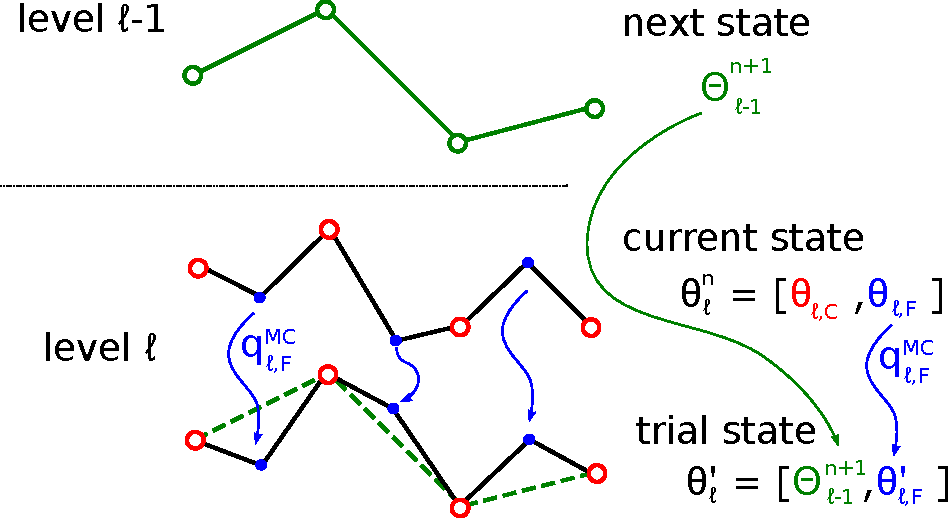
\includegraphics[width=0.6\linewidth]{\figdir/multilevel_paths.pdf}
    \caption{Multilevel sampling of paths}
    \label{fig:multilevel_path_sampling}
  \end{center}
\end{figure}

Coupling is ensured by drawing the coarse-level part of the proposal state from the distribution on the next-coarser level but the Metropolis acceptance step guarantees that the samples $\theta_\ell^n$ on level $\ell$ are indeed distributed according to $\pi^\ell$, which is necessary to make the estimator in Eq. (\ref{eqn:MLMCMCestimator}) unbiased.
%%%%%%%%%%%%%%%%%%%%%%%%%%%%%%%%%%%%%%%%%%%%%%%%%%%%%%%%%%%%%%%%%%%%%%%%%%%%
\subsubsection{Fine level sampling}\label{sec:fine_draw}
%%%%%%%%%%%%%%%%%%%%%%%%%%%%%%%%%%%%%%%%%%%%%%%%%%%%%%%%%%%%%%%%%%%%%%%%%%%%
As explained in Algorithm \ref{alg:MLMC_sampling}, the proposal $\theta'_{\ell,C}$ for the coarse modes on the fine level $\ell$ is obtained by using the next state on the coarse level $\ell-1$. A suitable proposal distribution $\theta'_{\ell,F}$ should ensure that the acceptance probability is high, i.e. it should pick points that are close to the correct distribution. For this, observe that the distribution for a fine point $X$ lying between two coarse points $X_-$ and $X_+$ is a conditional distribution given by
\begin{equation}
  p(X|X_-,X_+) = Z_{X_+,X_-}^{-1} \exp\left[
  - a \left(\frac{m_0}{2}\frac{(X-X_-)^2+(X_+-X)^2}{a^2}+V(X)\right)
  \right]\label{eqn:fine_proposal_exact}
\end{equation}
where $Z_{X_+,X_-}$ is an unknown normalisation constant which guarantees that the conditional distribution $p(X|X_-,X_+)$ is indeed a probability and integrates to one. Ideally we would like to sample from this distribution to pick the fine points between any two given coarse points but (a) we don't know the normalisation constant $Z(X_+,X_-)$ and (b) exact sampling from $p$ in Eq. (\ref{eqn:fine_proposal_exact}) is not possible, so we would need to to MCMC again.

However, as $a\rightarrow 0$ the first term in the exponential in Eq. (\ref{eqn:fine_proposal_exact}) dominates. It therefore makes sense to instead sample from the Gaussian free distribution
\begin{equation}
  p_{\text{free}}(X|X_-,X_+) = \sqrt{\frac{m_0}{\pi a}}\exp\left[-\frac{m_0}{a}\left(X-\frac{X_-+X_+}{2}\right)^2\right]
\end{equation}
Note that this has mean $\frac{1}{2}(X_-+X_+)$ and width $\sqrt{\frac{a}{2m_0}}$ and sampling from this is trivial since we can generate normally distributed random numbers. In summary, we draw the fine modes from
\begin{equation}
  \pi^\ell_{\text{free}}(\theta'_{\ell,F}|\theta'_{\ell,C}) =
  C_\ell
  \exp\left[-S^\ell_{\text{free}}[\theta'_\ell]\right]
\end{equation}
with
\begin{equation}
  S^\ell_\text{free}[\theta_\ell] = 
  -\frac{a_\ell m^{(\ell)}_0}{2}\sum_{j=0}^{M_\ell/2} \left(X^\ell_{2j+1}-\frac{X^\ell_{2j}+X^\ell_{2j+2}}{2}\right)^2
\end{equation}
and $C_\ell = \left(\frac{m^{(\ell)}_0}{\pi a_\ell}\right)^{M_{\ell}/4}$ is an irrelevant normalisation constant which cancels out in the end.
Using all this, we can express the ratio in Eq. (\ref{eqn:alpha_accept}) as
\begin{equation}
  \frac{\pi^\ell(\theta'_\ell)\pi^{\ell-1}(\theta_{\ell,C}^n)\pi^\ell_{\text{free}}(\theta_{\ell,F}^n|\theta_{\ell,C}^n)}{\pi^\ell(\theta_\ell^n)\pi^{\ell-1}(\theta'_{\ell,C})\pi^\ell_{\text{free}}(\theta'_{\ell,F}|\theta'_{\ell,C})}
  = \exp\left[-\delta S^{\ell}[\theta'_\ell,\theta^n_\ell]\right]
\end{equation}
with
\begin{equation}
  \delta S^\ell[\theta'_\ell,\theta^n_\ell] =
  S^\ell[\theta'_\ell] - S^\ell[\theta^n_\ell] +
  S^{\ell-1}[\theta^n_{\ell,C}] - S^{\ell-1}[\theta'_{\ell,C}] +
  S^{\ell}_{\text{free}}[\theta^n_{\ell}] - S^{\ell}_{\text{free}}[\theta'_{\ell}].
  \end{equation}
%%%%%%%%%%%%%%%%%%%%%%%%%%%%%%%%%%%%%%%%%%%%%%%%%%%%%%%%%%%%%%%%%%%%%%%%%%%%
\subsubsection{Coarse level sampling}
%%%%%%%%%%%%%%%%%%%%%%%%%%%%%%%%%%%%%%%%%%%%%%%%%%%%%%%%%%%%%%%%%%%%%%%%%%%%
Above we assumed that it is possible to sample independently from $\pi^{\ell-1}$. This can be achieved by using the above procedure to create two chains on each level $\ell$: (a) the chain $\theta_\ell$ which we will use together with the chain $\Theta_{\ell-1}$ to calculate $\hat{Y}_{\ell,N_\ell}^{MC}$ and (b) another chain $\Theta_{\ell}$, for which we only take every $k$-th sample where $k$ is large compared to the autocorrelation time. To a very good approximation this chain then samples from $\pi^\ell$. The procedure is shown schematically in Fig. \ref{fig:chains} and as the authors of \cite{Dodwell2015} remark, the bias error due to any remaining auto-correlation is small.
\begin{figure}
  \begin{center}
    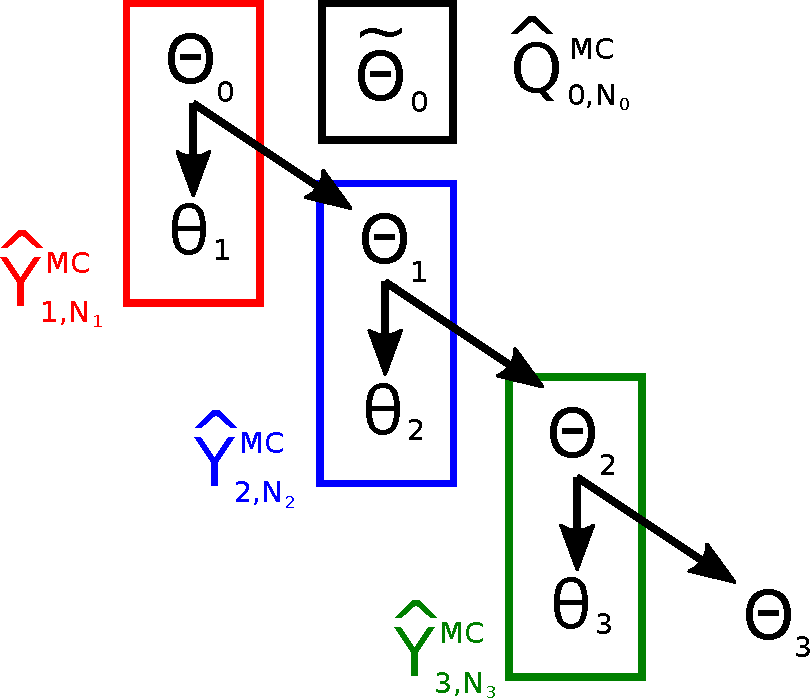
\includegraphics[width=0.3\linewidth]{\figdir/chains.pdf}
    \caption{Recursive construction of the chains $\{\theta_\ell^n\}_{n\in\mathbb{N}}$ and $\{\Theta_\ell^n\}_{n\in\mathbb{N}}$. The arrows indicate coupled sampling according to Algorithm \ref{alg:MLMC_sampling}.}
    \label{fig:chains}
  \end{center}
\end{figure}
%%%%%%%%%%%%%%%%%%%%%%%%%%%%%%%%%%%%%%%%%%%%%%%%%%%%%%%%%%%%%%%%%%%%%%%%%%%%
\subsection{Coarse graining and effective theories}\label{sec:coarse_graining}
%%%%%%%%%%%%%%%%%%%%%%%%%%%%%%%%%%%%%%%%%%%%%%%%%%%%%%%%%%%%%%%%%%%%%%%%%%%%
We now discuss the recursive construction of the coarse level theory in Eq. (\ref{eqn:MultilevelCoarseAction}). For the multilevel method to be effective, the coarse action has to be ``good'' in the sense that it accurately describes the coarse modes in the original model. Only then will the variance of the difference estimators $\hat{Y}^{MC}_{\ell,N_\ell}$ in Eq. (\ref{eqn:difference_estimator}) be small enough to satisfy the Complexity Theorem 3.4 in \cite{Dodwell2015}. We describe a recursive matching procedure for the construction of an effective coarse level theory.

Define the following \textit{generating functional}
\begin{equation}
  Z[J] = \int \mathcal{D}x(t)\;\exp\left[-S[x(t)]+\int_0^T J(t)x(t)\;dt \right]\label{eqn:generating_functional_cont}
\end{equation}
This can be seen as a response function for an external current $J(t)$.
$Z[J]$ allows the formal expression of expectation values as functional derivatives
\begin{equation}
\langle A[x(t)] \rangle = (Z[0])^{-1}A\left[\frac{\delta}{\delta J(t)}\right] Z[J]\Big|_{J=0}
\end{equation}
since
\begin{equation}
\frac{\delta J(t')}{\delta J(t)} = \delta(t'-t).
\end{equation}
For example, if $A[x(t)]=x(t_1)x(t_2)$ then
\begin{equation}
\langle x(t_1)x(t_2)\rangle = (Z[0])^{-1} \frac{\delta}{\delta J(t_1)}
\frac{\delta}{\delta J(t_2)} Z[J]\Big|_{J=0}
\end{equation}
In other words, the generating functional contains all useful information on the theory\footnote{In QFT one often works with the connected $n$-point functions
\begin{equation}
  \Gamma_c^{(n)} = \frac{\delta}{\delta J(t_1)}\dots\frac{\delta}{\delta J(t_n)} \log\left(Z[J]\right)_{J=0},\qquad\text{e.g.}\quad\Gamma_c^{(2)} = \langle x(t_1)x(t_2)\rangle-\langle x(t_1)\rangle\langle x(t_2)\rangle
\end{equation}}.

We can also write down the generating functional for the discrete theory as
\begin{equation}
  Z[\vec{J}] = \int d^{M}\vec{X} \exp\left[-S[\vec{X}]+\vec{J}^T\vec{X}\right]
\end{equation}
where now $J=(J_0,J_1,J_2,\dots,J_{M-1})$ is a $M$-dimensional vector.
To coarse-grain the theory, replace the state vector $\vec{X}=(X_0,X_1,X_2,\dots,X_{M-1})$ by the coarse vector
\begin{equation}
  \vec{X}^{(c)}=(X_0^{(c)},X_1^{(c)},\dots,X_{M/2}^{(c)}) = (X_0,X_2,X_4,\dots,X_{M/2})
\end{equation}
which only describes the path on the even lattice sites. 
There are two ways of writing down a coarse action:
\begin{itemize}
\item \textit{naive}. Simply take the action in Eq. (\ref{eqn:action_discrete}) with $2a$ instead of $a$, i.e.
  \begin{equation}
    S^{(c)}[\vec{X}^{(c)}] = \sum_{j=0}^{M/2} 2a \left(\frac{1}{2}m_0\frac{(X_{2j+1}-X_{2j})^2}{(2a)^2}+V(X_{2j})\right)
    \end{equation}
\item \textit{effective}. Construct the coarse action $S^{(c)}$ such that it has the same response to a coarse level current $J^{(c)}=(J_0^{(c)},J_1^{(c)},\dots,J_{M/2}^{(c)})$
  \begin{equation}
    Z^{(c)}[\vec{J}^{(c)}] = \int d^{M/2}\vec{X}^{(c)} \exp\left[-S^{(c)}[\vec{X}^{(c)}]+(\vec{J}^{(c)})^T\vec{X}^{(c)}\right] = Z[\hat{\vec{J}}^{(c)}]
  \end{equation}
where $\hat{J}^{(c)}=(J_0^{(c)},0,J_1^{(c)},0,\dots,J_{M/2}^{(c)},0)$, i.e. this is an external current on the fine grid which is only non-zero on the coarse level nodes\footnote{Actually, since normalisation factors cancel out, $Z^{(c)}[J^{(c)}]=C(a) Z[\hat{J}^{(c)}]$ where $C(a)$ is a constant is sufficient.}.
  This results in
  \begin{equation}
    S^{(c)}[\vec{X}^{(c)}] = -\log \left(\int d^{M/2}\vec{X}^{(f)}\; \exp\left[-S[\vec{X}]\right]\right)\qquad\text{where $d^{M/2}\vec{X}^{(f)}=dX_1\;dX_3\;\dots\;dX_{M-1}$}
  \end{equation}
  In other words, the effective action is obtained by integrating out all odd modes $X^{(f)}$ which are not represented on the coarse grid.
\end{itemize}
Note that sampling from the effective action will give coarse level samples which have exactly the same distribution as the coarse modes in a fine level sample.
Calculation of the effective action is only possible in exceptional cases (for example, the harmonic oscillator, see Appendix \ref{sec:harmonic_oscillator_effective}). In other cases it will be a very complicated object. However, it can be calculated approximately, and will lead to a much better coarse level model than the naive approach which fails to represent fluctuations of size $\sim a$.

For example, consider the quartic oscillator, $V(x) = \frac{1}{2}\mu_0 x^2 + \frac{1}{4}\lambda_0 x^4$. In this case the fine-level and an approximate coarse-grained action would be
\begin{equation}
  \begin{aligned}
  S[\vec{X}] = \sum_{j=0}^{M-1} a \left(\frac{1}{2}m_0\frac{(X_{j+1}-X_{j})^2}{a^2}+\frac{1}{2}\mu_0 X_{j}^2 + \frac{1}{4}\lambda_0 X_{j}^4\right)\\
  S^{(c)}[\vec{X}^{(c)}] = \sum_{j=0}^{M/2-1} 2a \left(\frac{1}{2}m^{(c)}_0\frac{(X_{2j+1}-X_{2j})^2}{(2a)^2}+\frac{1}{2}\mu_0^{(c)}X_{2j}^2 + \frac{1}{4}\lambda_0^{(c)} X_{2j}^4\right)
  \end{aligned}
\end{equation}
where
\begin{xalignat}{3}
  m_0^{(c)} &= m_0^{(c)}(m_0,\mu_0,\lambda_0), &
  \mu_0^{(c)} &= \mu_0^{(c)}(m_0,\mu_0,\lambda_0), &
  \lambda_0^{(c)} &= \lambda_0^{(c)}(m_0,\mu_0,\lambda_0)\label{eqn:renormalised_couplings}
\end{xalignat}
can be calculated using perturbation theory.

For example, for the quartic oscillator we can define a potential on level $\ell$ by
\begin{equation}
  V^\ell(x) = \frac{1}{2}\mu^{(\ell)}_0 x^2 + \frac{1}{4}\lambda_0^{(\ell)} x^4
\end{equation}
and then calculate mass $m_0^{(\ell)}$ and coupling constants $\mu_0^{(\ell)}$, $\lambda_0^{(\ell)}$ perturbatively as in Eq. (\ref{eqn:renormalised_couplings})
\begin{xalignat}{3}
  m_0^{(\ell-1)} &= m_0^{(\ell-1)}(m_0^{(\ell)},\mu_0^{(\ell)},\lambda_0^{(\ell)}), &
  \mu_0^{(\ell-1)} &= \mu_0^{(\ell-1)}(m_0^{(\ell)},\mu_0^{(\ell)},\lambda_0^{(\ell)}), &
  \lambda_0^{(\ell-1)} &= \lambda_0^{(\ell-1)}(m_0^{(\ell)},\mu_0^{(\ell)},\lambda_0^{(\ell)})
\end{xalignat}
starting with
\begin{xalignat}{3}
  m_0^{(L)} &= m_0, &
  \mu_0^{(L)} &= \mu_0, &
  \lambda_0^{(L)} &= \lambda_0.
\end{xalignat}


%%%%%%%%%%%%%%%%%%%%%%%%%%%%%%%%%%%%%%%%%%%%%%%%%%%%%%%%%%%%%%%%%%%%%%%%%%%%
\subsection{Quantum field theory}\label{sec:QFT}
%%%%%%%%%%%%%%%%%%%%%%%%%%%%%%%%%%%%%%%%%%%%%%%%%%%%%%%%%%%%%%%%%%%%%%%%%%%%
The quantum theory above is one-dimensional, i.e. there is only a lattice in the time-direction. In the continuum a configuration of the system is described by a path $x(t)$. In quantum field theory this is replaced by a field $\phi(\vec{x},t)$ which is a function of the independent space-time variables $\vec{x}\in\mathbb{R}^3$ and $t\in\mathbb{R}$, and hence the theory becomes four-dimensional. However, the same ideas as above apply. The Generating functional is now written as an integral over field configurations
\begin{equation}
Z[J] = \int\mathcal{D}\phi(\vec{x},t)\;\exp\left[-S[\phi(\vec{x},t)]+\int
  J(\vec{x},t)\phi(\vec{x},t)\;d^3\vec{x}\;dt)\right]
\end{equation}
Where the action $S[\phi(\vec{x},t)]$ is an integral over four-dimensional space-time. Discretisation works exactly as above, but now we have a four-dimensional space-time lattice. Coarse-graining by removing lattice sites will be much more effective in four dimensions since the number of points is reduced by a factor 16 instead of 2.
%%%%%%%%%%%%%%%%%%%%%%%%%%%%%%%%%%%%%%%%%%%%%%%%%%%%%%%%%%%%%%%%%%%%%%%%%%%%
\subsubsection{Connections to statistical physics}
%%%%%%%%%%%%%%%%%%%%%%%%%%%%%%%%%%%%%%%%%%%%%%%%%%%%%%%%%%%%%%%%%%%%%%%%%%%%

%%%%%%%%%%%%%%%%%%%%%%%%%%%%%%%%%%%%%%%%%%%%%%%%%%%%%%%%%%%%%%%%%%%%%%%%%%%%
\section{Workplan}
%%%%%%%%%%%%%%%%%%%%%%%%%%%%%%%%%%%%%%%%%%%%%%%%%%%%%%%%%%%%%%%%%%%%%%%%%%%%
Lattice QCD is a highly complicated theory, in particular it is invariant under non-trivial local $SU(3)$ gauge transformations, i.e. there are certain equivalent field configurations which have exactly the same action. This as to be taken into account during the sampling process. Perturbative calculations of the lattice are also non-trivial. We therefore propose to approach the problem in several stages of increasing complexity:
%%%%%%%%%%%%%%%%%%%%%%%%%%%%%%%%%%%%%%%%%%%%%%%%%%%%%%%%%%%%%%%%%%%%%%%%%%%%
\subsection{Simple quantum mechanical systems}
%%%%%%%%%%%%%%%%%%%%%%%%%%%%%%%%%%%%%%%%%%%%%%%%%%%%%%%%%%%%%%%%%%%%%%%%%%%%
To start with, consider one-dimensional quantum system such as the quadratic or quartic oscillator; an elementary discussion of Monte Carlo sampling for this system can be found in \cite{Creutz1981}. For the quadratic oscillator all integrals are Gaussian and can be solved exactly (including both finite-volume and finite-size effects), which allows comparison to known theory. In this case it is also possible to sample directly (avoiding MCMC), which could lead to further simplifications.
Next, consider the quartic oscillator or a slightly perturbed harmonic oscillator, i.e. systems for which there are no analytical results. The effective action in this case can be calculated with perturbation theory, or one could just use the original action at half the lattice spacing and see what the difference in performance is. The gains in those one-dimensional systems are likely smaller, but could give a guide as to what can be achieved in higher dimensions.
%%%%%%%%%%%%%%%%%%%%%%%%%%%%%%%%%%%%%%%%%%%%%%%%%%%%%%%%%%%%%%%%%%%%%%%%%%%%
\subsection{Quantum Field Theories}
%%%%%%%%%%%%%%%%%%%%%%%%%%%%%%%%%%%%%%%%%%%%%%%%%%%%%%%%%%%%%%%%%%%%%%%%%%%%
Again consider theories of increasing complexity:
\begin{enumerate}
\item \textit{Free scalar field theory of a massive particle}. Again all integrals are Gaussian and can be solved in principle, allowing a comparison to theory. Obviously this case is a but boring since there is no renormalisation
\item \textit{The non-linear sigma model}. Consider this model in $d=2$ dimensions where it is asymptotically free if the number $N_{\text{spin}}$ of spin components is three or more. In higher dimensions there also appears to be a non-trivial critical point, which might be worth studying and this could potentially be analysed asymptotically for $N_{\text{spin}}\gg 1$
  \item \textit{Lattice QCD}. Study full blown QCD, in particular think about the implications of the $SU(3)$ symmetry for Multilevel Monte Carlo sampling
\end{enumerate}
%%%%%%%%%%%%%%%%%%%%%%%%%%%%%%%%%%%%%%%%%%%%%%%%%%%%%%%%%%%%%%%%%%%%%%%%%%%%
\subsection{Code development}
%%%%%%%%%%%%%%%%%%%%%%%%%%%%%%%%%%%%%%%%%%%%%%%%%%%%%%%%%%%%%%%%%%%%%%%%%%%%
Implement the techniques by either developing a bespoke multilevel software for lattice QCD or incorporate it into existing codes such as CHROMA \cite{Edwards2005}. Run code on clusters to obtain calculations of benchmark quantities to higher accuracy. \note{Link to CRAY/GW4 Isambard?}
%%%%%%%%%%%%%%%%%%%%%%%%%%%%%%%%%%%%%%%%%%%%%%%%%%%%%%%%%%%%%%%%%%%%%%%%%%%%
\section{Tasks/Questions}
%%%%%%%%%%%%%%%%%%%%%%%%%%%%%%%%%%%%%%%%%%%%%%%%%%%%%%%%%%%%%%%%%%%%%%%%%%%%
\begin{itemize}
  \item Understand Hybrid Monte Carlo and how it relates to multilevel sampling. For example, does the hierarchical sampling in Multilevel MCMC make Hybrid MC for the suggesting the trial state unnecessary?
  \item Understand the implications of $SU(3)$ invariance for coupling between levels
  \item Multilevel sampling is dependent on the QoI, but traditionally lattice configurations are just generated and then used for several QoIs. Is this a limitation of the multilevel approach?
\item For asymptotically free theories such as QCD, the difference between the fine and coarse theories on subsequent levels becomes smaller. Does this lead to some soft of ``superconvergence'', since the variance decays more rapidly?
\end{itemize}
\appendix
%%%%%%%%%%%%%%%%%%%%%%%%%%%%%%%%%%%%%%%%%%%%%%%%%%%%%%%%%%%%%%%%%%%%%%%%%%%%
\section{Harmonic Oscillator}\label{sec:harmonic_oscillator}
%%%%%%%%%%%%%%%%%%%%%%%%%%%%%%%%%%%%%%%%%%%%%%%%%%%%%%%%%%%%%%%%%%%%%%%%%%%%
For a harmonic oscillator with $V(x) = \frac{1}{2}m_0\mu^2 x^2$ the 
action can be written as
\begin{equation}
  S[X] = \sum_{j=0}^{M} a \left( \frac{1}{2}m_0 \frac{(X_{j+1}-X_j)^2}{a^2}+\frac{1}{2}m_0\mu^2 X_j^2\right) := \frac{1}{2}X^T G X\label{eqn:ho_action}
\end{equation}
The generating functional is a Gaussian integral and can be evaluated exactly
\begin{equation}
  Z[\vec{J}] = \int d^M\vec{x}\;\exp\left[-\frac{1}{2}\vec{X}^T G \vec{X} + \vec{J}^T \vec{X}\right]
  \end{equation}
with the $M\times M$ correlation matrix
\begin{equation}
  G = \begin{pmatrix}
    d & c & & \dots & & c\\
    c & d & c & &\\
    & c & d & c & & \\
    \vdots & & & \ddots & & \vdots\\
    & & & c & d & c\\
        c & & \dots & & c & d\\
  \end{pmatrix}\label{eqn:HO_G}
\end{equation}
with
\begin{xalignat}{2}
d &= am_0\mu^2 + 2m_0/a, & c &= -m_0/a\label{eqn:c_d_def}.
\end{xalignat}
This implies that
\begin{equation}
  \log\left(Z[\vec{J}]\right) = C(a) + \frac{1}{2}\vec{J}^T G^{-1} \vec{J}
\end{equation}
where $C(a)$ is a constant.
This immediately allows the calculation of
\begin{equation}
  \langle X^2\rangle = \langle X_j^2 \rangle = \left(G^{-1}\right)_{jj} = \frac{1}{M}\operatorname{trace}\left(G^{-1}\right) = \sum_{k=0}^{N-1} \left(m_0\mu^2 + \frac{4m_0\sin^2(ka/2)}{a^2}\right)^{-1}
\end{equation}
In \cite{Creutz1981} the exact value of $\langle X^2 \rangle$ is calculated as
\begin{equation}
  \langle X^2\rangle = \frac{1}{2m_0\mu\sqrt{1+\frac{a^2\mu^2}{4}}}\cdot\frac{1+R^M}{1-R^M}\label{eqn:Xsquared_exact}
\end{equation}
with
\begin{equation}
R = 1+\frac{a^2\mu^2}{2}-a\mu\sqrt{1+\frac{a^2\mu^2}{4}}.
\end{equation}
Note that the expression in Eq. (\ref{eqn:Xsquared_exact}) contains both finite resolution ($a>0$) and finite volume ($L<\infty$) effects. In the continuum- and infinite-volume- limit the standard result (see e.g. Section 2.3 in \cite{Sakurai1994}) is recovered
\begin{equation}
\langle X^2\rangle\;\; \underset{a\rightarrow 0}{\longrightarrow}\;\;
\frac{1}{2m_0\mu}\frac{1+e^{-\mu T}}{1-e^{-\mu T}}
=\frac{1}{2m_0\mu}\coth\left(\frac{1}{2}\mu T\right)=\langle X^2\rangle_{\text{cont.}}
\;\; \underset{T\rightarrow \infty}{\longrightarrow}\;\;\frac{1}{2m_0 \mu}.\label{eqn:Xsquared_continuum}
\end{equation}
Taylor-expanding we can also calculate the leading-order corrections in the lattice spacing as
\begin{equation}
  \langle X^2\rangle = \langle X^2\rangle_{\text{cont.}} - \frac{\mu a^2}{16 m_0}\left(\coth\left(\rho\right)-\frac{\rho}{3\sinh^2\left(\rho\right)}\right)
  \qquad\text{with $\rho=\frac{\mu T}{2}$} \label{eqn:finitea_corrections}
\end{equation}
Observe that since the ground state energy is $E_0=\frac{1}{2}\mu$, fine volume effects are indeed exponentially expressed by
\begin{equation}
e^{-2E_0T} = \exp\left[-C\cdot \text{(ground state energy)}\times\text{(simulation volume)}\right]
\end{equation}
as claimed above. Upon suitable scaling $\langle X^2\rangle$ is related to the ground state energy. Note that due to translational invariance $\langle X_j^2\rangle =\langle X_0^2\rangle$ and $\left(G^{-1}\right)_{jj}=\left(G^{-1}\right)_{00}=\frac{1}{M}\operatorname{trace}\left(G^{-1}\right)$ for any $j=0,\dots,M-1$.
%%%%%%%%%%%%%%%%%%%%%%%%%%%%%%%%%%%%%%%%%%%%%%%%%%%%%%%%%%%%%%%%%%%%%%%%%%%%
\subsection{Cost analysis}
%%%%%%%%%%%%%%%%%%%%%%%%%%%%%%%%%%%%%%%%%%%%%%%%%%%%%%%%%%%%%%%%%%%%%%%%%%%%
For the single level method we find that the bias $\delta E_{\text{bias}}$ of $\langle X^2\rangle$ decreases quadratically with the lattice spacing $a=T/M$
\begin{equation}
  \delta E_{\text{bias}}(M) \approx \frac{C_{\text{bias}}}{M^2}
\end{equation}
where $C_{\text{bias}}$ is a numerical constant that depends on $m_0$, $\mu^2$ and $T$. It can read off from Eq. (\ref{eqn:finitea_corrections}) as
\begin{equation}
  C_{\text{bias}} = \frac{\mu T^2}{16 m_0}\left(\coth\left(\rho\right)-\frac{\rho}{3\sinh^2\left(\rho\right)}\right)
  \qquad\text{with $\rho=\frac{\mu T}{2}$}.
\end{equation}
We also know from the law of large numbers that the squared sampling error is proportional to the variance $V$ of the quantity of interest and decrases linearly with the number of samples $N$
\begin{equation}
  \left(\delta E^{\text{StMC}}_{\text{sampling}}(N)\right)^2 \approx \frac{V}{N}
\end{equation}
with $V$ the variance of $X^2$. Since everything is Gaussian, we know that $V=2\langle X^2\rangle^2$ which depends on $a$, $m_0$, $\mu^2$ and $T$. However, for the following analysis we use the continuum limit ($a=0$) of $\langle X^2\rangle$ given in Eq. (\ref{eqn:Xsquared_continuum}). To reduce the total root mean square error below a tolerance $\epsilon$, pick $N$ and $M$ such that
\begin{xalignat}{2}
  \left(\delta E_{\text{bias}}(M)\right)^2 &= \frac{\epsilon^2}{2}, &
    \left(\delta E^{\text{StMC}}_{\text{sampling}}(N)\right)^2 &= \frac{\epsilon^2}{2}.
\end{xalignat}
This choice results in a cost of
\begin{equation}
  \text{Cost}^{\text{StMC}}(\epsilon) = N\cdot M = 2^{5/4}C_{\text{bias}}^{1/2} V\epsilon^{-5/2}
\end{equation}
For the multilevel method with $L+1$ levels such that $M_\ell=2^\ell M_0$ on level $\ell$ the bias error is given by the bias on the finest level
\begin{equation}
  \delta E_{\text{bias}}(M_L) = \frac{C_{\text{bias}}}{M_L^2} = \frac{C_{\text{bias}}}{M_0^2} 4^{-L}  \label{eqn:MLMC_bias}
\end{equation}
Using $N_\ell$ samples on level $\ell$ the total squared sampling error is
\begin{equation}
  \left(\delta E^{\text{MLMC}}_{\text{sampling}}(\{N_\ell\})\right)^2 \approx \frac{V}{N_0} + \sum_{\ell=1}^{L} \frac{\delta V_\ell}{N_\ell}
  \approx \frac{V}{N_0} + \frac{C_{\delta V}}{M_0} \sum_{\ell=1}^{L} \frac{2^{-\ell}}{N_\ell}.
  \label{eqn:MLMC_sampling_error}
\end{equation}
Here we assumed that the variance $\delta V_\ell$ of the difference of the QoI on two subsequent levels $\ell$ and $\ell-1$ decays as
\begin{equation}
  \delta V_\ell = \frac{C_{\delta V}}{M_{\ell}} = \frac{C_{\delta V}}{M_0} 2^{-\ell}
\end{equation}
as is confirmed by the numerical experiments.
If we assume that calculating a sample for the difference estimator on two subsequent levels is about twice as expensive as calculating a sample on one level, the total cost is
\begin{equation}
  \text{Cost}^{\text{MLMC}}(\{N_\ell\}) = M_0N_0 + 2\sum_{\ell=1}^{L} M_\ell N_\ell =
  M_0 \left(N_0 + 2\sum_{\ell=1}^{L} 2^\ell N_\ell\right)
\end{equation}
Minimising the cost under the constraint that both the square of the bias-error in Eq. (\ref{eqn:MLMC_bias}) and the squared sampling-error in Eq. (\ref{eqn:MLMC_sampling_error}) do not exceed $\epsilon^2/2$ gives
\begin{equation}
  \begin{aligned}
    N_0 &= \frac{2}{\epsilon^2}\left(V+\sqrt{\frac{2VC_{\delta V}}{M_0}}L\right)\\
    N_{\ell} &= \frac{2}{\epsilon^2}\left(\sqrt{\frac{V C_{\delta V}}{2M_0}}+\frac{C_{\delta V}}{M_0}L\right)2^{-\ell}
  \end{aligned}
\end{equation}
Given a tolerance $\epsilon$, the number of levels $L$ can be found using Eq. (\ref{eqn:MLMC_bias}) as
\begin{equation}
  L = \frac{1}{4} \left(1+\log_2\left(C_{\text{bias}}^2M_0^{-4}\right)\right)-\frac{1}{2}\log_2(\epsilon)
\end{equation}
This results in a total cost of
\begin{equation}
  \text{Cost}^{\text{MLMC}} = \frac{4C_{\delta V}}{\epsilon^2}\left(L+\sqrt{\frac{M_0V}{2C_{\delta V}}}\right)^2 \rightarrow C_{\delta V}\epsilon^{-2}|\log(\epsilon)|^2\quad\text{as $\epsilon\rightarrow 0$}.
\end{equation}
We can calculate the costs of the standard- and multilevel-Monte Carlo method if we know the numerical values of $C_{\text{bias}}$, $V$ and $C_{\delta V}$.
%%%%%%%%%%%%%%%%%%%%%%%%%%%%%%%%%%%%%%%%%%%%%%%%%%%%%%%%%%%%%%%%%%%%%%%%%%%%
\subsection{Effective theory}\label{sec:harmonic_oscillator_effective}
%%%%%%%%%%%%%%%%%%%%%%%%%%%%%%%%%%%%%%%%%%%%%%%%%%%%%%%%%%%%%%%%%%%%%%%%%%%%
To construct the effective theory, rearrange the state vector $X$ as
\begin{equation}
X = (X_0,X_2,X_4,\dots,X_{M/2};X_1,X_3,\dots,X_{M/2+1}) := (X^{(c)},X^{(f)})
\end{equation}
This results in
\begin{equation}
X^T G X = \left(\left(X^{(c)}\right)^T,\left(X^{(f)}\right)^T\right) 
\begin{pmatrix}
D & C^T\\
C & D
\end{pmatrix}
\begin{pmatrix}
X^{(c)}\\X^{(f)}
\end{pmatrix}
\end{equation}
with
\begin{xalignat}{2}
D &= \begin{pmatrix}
d & \\
  & d \\
  & & \ddots \\
  & & & d
\end{pmatrix},&
C &= \begin{pmatrix}
c & c \\
  & c & c\\
  & & c & c\\
  & & & \ddots & \ddots\\
  & & & & c & c\\
c & & & &   & c
\end{pmatrix}
\end{xalignat}
with $c$ and $d$ as defined in Eq. (\ref{eqn:c_d_def}).
Then integrate out the fine (odd) modes to obtain by completing the square in the exponential and carrying out the Gaussian integral over the fine modes:
\begin{equation}
\begin{aligned}
Z^{(c)}[J^{(c)}] = Z[J^{(c)}] &= \int d^MX \exp\Big[-\frac{1}{2}\Big(
\left(X^{(c)}\right)^T D X^{(c)} +
\left(X^{(c)}\right)^T C^T X^{(f)} +
\left(X^{(f)}\right)^T C X^{(c)}\\
&\qquad\qquad\qquad+\;\;
\left(X^{(c)}\right)^T D X^{(c)}
\Big)+\left(J^{(c)}\right)^T X^{(c)}\Big]\\
&= C(a)\int d^{M/2} X^{(c)}\exp\left[-\frac{1}{2}\left(X^{(c)}\right)^TG^{(c)}X^{(c)}+\left(J^{(c)}\right)X^{(c)}\right]
\end{aligned}
\end{equation}
Here $G^{(c)}$ is the Schur-complement of the matrix $G$,
\begin{equation}
  G^{(c)} = D - C D^{-1} C^T
\end{equation}
Furthermore, it is easy to see that $G^{(c)}$ has exactly the same structure as $G$ in Eq. (\ref{eqn:HO_G}), but with $a\mapsto 2a$, $m_0\mapsto m_0^{(c)}$, $\mu\mapsto \mu^{(c)}$. The coarse level couplings are
\begin{xalignat}{2}
m_0^{(c)} &= m_0\left(1+\frac{a^2\mu^2}{2}\right)^{-1}, &
\left(\mu^{(c)}\right)^2 &= \mu^2 \left(1+\frac{a^2\mu^2}{4}\right)
\end{xalignat}
Hence, the coarse level action also has the same structure as in Eq. (\ref{eqn:ho_action}) and can be written as 
\begin{equation}
  S^{(c)}[X^{(c)}] = \sum_{j=0}^{M/2} 2a \left( \frac{1}{2}m^{(c)}_0 \frac{(X^{(c)}_{j+1}-X^{(c)}_j)^2}{(2a)^2}+\frac{1}{2}m_0^{(c)}\left(\mu^{(c)}\right)^2 \left(X^{(c)}_j\right)^2\right)
\end{equation}
In Fig. \ref{fig:harmonic_oscillator_flow} we show the evolution of the coupling constants as a function of $a$, where we've chosen $m_0(a^*)=10$ and $\mu^2(a^*) = 6$ and $a^*\ll 1$ is the grid spacing at which we want to carry out our simulation.
Note that for $a\sim 1$ taking the naive action with $m_0=m_0(a^*)$, $\mu^2=\mu^2(a^*)$ is likely to lead to bad results.
\begin{figure}
\begin{center}
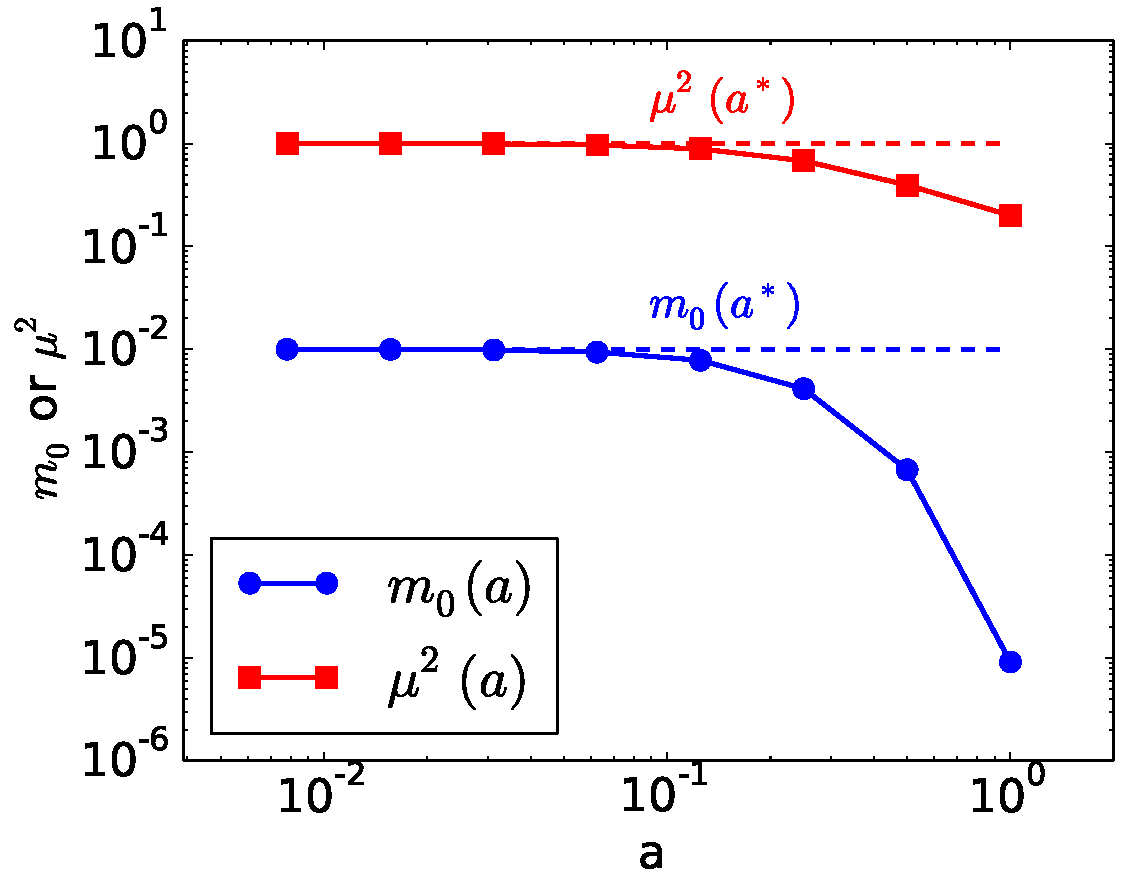
\includegraphics[width=0.5\linewidth]{\figdir/harmonic_oscillator_flow.pdf}
\caption{Evolution of coupling constants $m_0$ and $\mu$ as a function of the lattice spacing $a$ for the harmonic oscillator.}
\label{fig:harmonic_oscillator_flow}
\end{center}
\end{figure}

%%%%%%%%%%%%%%%%%%%%%%%%%%%%%%%%%%%%%%%%%%%%%%%%%%%%%%%%%%%%%%%%%%%%%%%%%%%%%
% B I B L I O G R A P H Y
%%%%%%%%%%%%%%%%%%%%%%%%%%%%%%%%%%%%%%%%%%%%%%%%%%%%%%%%%%%%%%%%%%%%%%%%%%%%%
\bibliographystyle{unsrt}
\bibliography{plan}
\end{document}
